\documentclass{article}
\usepackage[utf8]{inputenc}
\usepackage{amsmath}
\usepackage{amsfonts}
\usepackage{amssymb}
\usepackage{url}
\usepackage{cite}
\usepackage{caption}
\usepackage{array}       
\usepackage[utf8]{inputenc}
\usepackage{longtable}
\usepackage{geometry}
\usepackage{tabularx}
\usepackage{graphicx}
\usepackage{listings}
\usepackage{xcolor}
\usepackage{longtable} 

\lstset{
	basicstyle=\ttfamily\small,        % Usar fuente tipo monoespaciada, más pequeña
	numbers=left,                      % Numerar las líneas a la izquierda
	numberstyle=\tiny\color{gray},     % Estilo de los números de línea
	stepnumber=1,                      % El número de pasos para la numeración
	numbersep=5pt,                     % Separación entre números y código
	backgroundcolor=\color{white},     % Color de fondo blanco
	showspaces=false,                  % No mostrar los espacios como '·'
	showstringspaces=false,            % No mostrar los espacios en las cadenas
	showtabs=false,                    % No mostrar las tabulaciones
	frame=single,                      % Enmarcar el código
	rulecolor=\color{black},           % Color del marco
	breaklines=true,                   % Ajuste automático de las líneas largas
	breakatwhitespace=true,            % Romper las líneas solo en espacios
	postbreak=\mbox{\textcolor{red}{$\hookrightarrow$}\space}, % Mostrar una flecha cuando una línea se rompe
	captionpos=b,                      % Posición de la leyenda abajo
	escapeinside={\%*}{*)},            % Escapar para insertar código LaTeX dentro del código
	morekeywords={*,...}               % Puedes añadir más palabras clave si es necesario
}

\title{\textbf{Capítulo 2: Optimización Estocástica: Algoritmos y sus Aplicaciones}}
\author{}
\date{}

\begin{document}
	
\maketitle
	En este capítulo se describen los algoritmos estocásticos utilizados en la optimización de modelos de ciencia de datos, particularmente en problemas de gran escala.
	
	\section*{2.1 Descenso de Gradiente Estocástico (SGD)}
	
     El \textbf{Descenso de Gradiente Estoc\'astico (SGD)} es un m\'etodo iterativo ampliamente utilizado en la optimizaci\'on de modelos de aprendizaje autom\'atico. A diferencia del \textit{Descenso de Gradiente por Lote}, donde el gradiente de la funci\'on de costo se calcula con todos los datos, el SGD actualiza los par\'ametros del modelo utilizando un \textit{\'unico} ejemplo o un mini-lote en cada iteraci\'on. Esto reduce la carga computacional y permite entrenar modelos en grandes conjuntos de datos con mayor eficiencia (Yan et al., 2018; Gadat et al., 2018).
     
     \subsection*{2.11 Fundamentos Matem\'aticos de SGD}
     
     La actualizaci\'on de par\'ametros en \textbf{SGD} se realiza mediante la regla:
     
     \begin{equation}
     	\theta_{t+1} = \theta_t - \eta \nabla_{\theta} L(\theta_t; x_i, y_i)
     \end{equation}
     
     Donde:
     \begin{itemize}
     	\item $\theta_t$ son los par\'ametros del modelo en la iteraci\'on $t$.
     	\item $\eta$ es la \textbf{tasa de aprendizaje}.
     	\item $\nabla_{\theta} L(\theta_t; x_i, y_i)$ es el gradiente de la funci\'on de p\'erdida respecto a $\theta$, evaluado en un ejemplo de entrenamiento $(x_i, y_i)$.
     \end{itemize}
     
     SGD es una variante eficiente para problemas de optimizaci\'on convexa y no convexa, y su convergencia ha sido ampliamente estudiada en diferentes escenarios (Orvieto et al., 2020).
     
     \subsection*{2.1.2 Propiedades y Convergencia}
     
     SGD tiene ventajas en t\'erminos de escalabilidad, pero introduce \textbf{oscilaciones en la convergencia} debido a la naturaleza estoc\'astica de la actualizaci\'on de gradientes. Se han desarrollado t\'ecnicas para mejorar su estabilidad, como:
     
     \begin{enumerate}
     	\item \textbf{Decaimiento de la tasa de aprendizaje}: Reducir $\eta$ con el tiempo ayuda a estabilizar la convergencia.
     	\item \textbf{SGD con Momento}: Se introduce una variable de memoria para suavizar las actualizaciones:
     	\begin{equation}
     		v_{t+1} = \beta v_t + (1 - \beta) \nabla_{\theta} L(\theta_t; x_i, y_i)
     	\end{equation}
     	\begin{equation}
     		\theta_{t+1} = \theta_t - \eta v_{t+1}
     	\end{equation}
     	Donde $v_t$ es el \textit{momento} acumulado y $\beta$ controla su efecto (Can et al., 2019).
     \end{enumerate}
     
     \subsection*{2.1.3 Variantes de SGD}
     
     \begin{itemize}
     	\item \textbf{SGD con Mini-lotes}: Usa peque\~nos subconjuntos de datos en cada actualizaci\'on en lugar de ejemplos individuales, logrando un equilibrio entre estabilidad y velocidad (Bottou, 2010).
     	\item \textbf{SGD Adaptativo}: M\'etodos como \textit{Adam, RMSProp y Adagrad} ajustan din\'amicamente la tasa de aprendizaje para cada par\'ametro, mejorando la optimizaci\'on en problemas no convexos (Kingma \& Ba, 2015).
     \end{itemize}
     
     \subsection*{2.1.4 Aplicaciones en Ciencia de Datos}
     
     SGD es utilizado en m\'ultiples \'areas:
     
     \begin{itemize}
     	\item \textbf{Redes Neuronales}: Es la base del entrenamiento en redes profundas como CNNs y RNNs.
     	\item \textbf{Optimizaci\'on en Grandes Datos}: Aplicado en modelos de regresi\'on log\'istica, SVMs y sistemas de recomendaci\'on.
     	\item \textbf{Procesamiento de Lenguaje Natural}: Modelos de embeddings como Word2Vec y BERT usan SGD para ajustar pesos de redes neuronales (Goodfellow et al., 2016).
     \end{itemize}
	
	
	\subsection*{2.1.5 Ejemplo}
	
\subsubsection*{1. Formulación Principal}

El \textbf{descenso de gradiente estocástico (SGD)} es un método iterativo de optimización que ajusta los parámetros de un modelo de manera progresiva utilizando una muestra aleatoria en cada actualización. En el caso de la \textbf{regresión lineal}, la función de pérdida es el \textbf{error cuadrático medio (MSE)}:

\[
L(\theta) = \frac{1}{n} \sum_{i=1}^{n} (y_i - \theta_0 - \theta_1 x_i)^2
\]

Donde:  
\begin{itemize}
	\item \( n \) es el número de muestras,  
	\item \( x_i \) y \( y_i \) son las características y etiquetas de los datos de entrenamiento,  
	\item \( \theta_0 \) y \( \theta_1 \) son los parámetros del modelo (intercepto y pendiente).  
\end{itemize}

El \textbf{descenso de gradiente estocástico} actualiza los parámetros de la siguiente manera:

\[
\theta_0^{t+1} = \theta_0^t - \eta \cdot \frac{\partial L}{\partial \theta_0}
\]

\[
\theta_1^{t+1} = \theta_1^t - \eta \cdot \frac{\partial L}{\partial \theta_1}
\]

Los gradientes se calculan a partir de un único ejemplo \( (x_i, y_i) \):

\[
\frac{\partial L}{\partial \theta_0} = -2 (y_i - \theta_0 - \theta_1 x_i)
\]

\[
\frac{\partial L}{\partial \theta_1} = -2 (y_i - \theta_0 - \theta_1 x_i) x_i
\]

\subsubsection*{2. Enunciado del Problema}

Se desea ajustar un modelo de \textbf{regresión lineal} utilizando el método de \textbf{descenso de gradiente estocástico (SGD)}. Para ello, se utilizará el siguiente conjunto de datos:

\begin{table}[h]
	\centering
	\begin{tabular}{|c|c|}
		\hline
		\( x \) & \( y \) \\
		\hline
		1 & 2 \\
		2 & 2.8 \\
		3 & 3.6 \\
		\hline
	\end{tabular}
	\caption{Datos de entrenamiento}
\end{table}

El modelo a ajustar es de la forma:

\[
y = \theta_0 + \theta_1 x
\]

Se trabajará con una \textbf{tasa de aprendizaje} de \( \eta = 0.1 \) y se realizarán tres iteraciones iniciales de \textbf{SGD} para observar cómo evolucionan los parámetros \( \theta_0 \) y \( \theta_1 \).

\subsubsection*{3. Datos Iniciales}

\begin{itemize}
	\item \textbf{Valores iniciales de los parámetros:} \( \theta_0 = 0 \), \( \theta_1 = 0 \)
	\item \textbf{Tasa de aprendizaje:} \( \eta = 0.1 \)
	\item \textbf{Datos de entrenamiento:}
	\begin{itemize}
		\item \( (x_1, y_1) = (1,2) \)
		\item \( (x_2, y_2) = (2,2.8) \)
		\item \( (x_3, y_3) = (3,3.6) \)
	\end{itemize}
\end{itemize}

\subsubsection*{4. Resolución Paso a Paso}

\textbf{Iteración 1 (usando \( x_1 = 1, y_1 = 2 \))}

\begin{enumerate}
	\item \textbf{Cálculo del error:}
	\[
	e = y_1 - (\theta_0 + \theta_1 x_1) = 2 - (0 + 0 \cdot 1) = 2
	\]
	
	\item \textbf{Cálculo de los gradientes:}
	\[
	\frac{\partial L}{\partial \theta_0} = -2 (2) = -4
	\]
	
	\[
	\frac{\partial L}{\partial \theta_1} = -2 (2) (1) = -4
	\]
	
	\item \textbf{Actualización de parámetros:}
	\[
	\theta_0^{(1)} = 0 - (0.1)(-4) = 0.4
	\]
	
	\[
	\theta_1^{(1)} = 0 - (0.1)(-4) = 0.4
	\]
\end{enumerate}

\textbf{Iteración 2 (usando \( x_2 = 2, y_2 = 2.8 \))}

\begin{enumerate}
	\item \textbf{Cálculo del error:}
	\[
	e = y_2 - (\theta_0 + \theta_1 x_2) = 2.8 - (0.4 + 0.4 \cdot 2) = 1.6
	\]
	
	\item \textbf{Cálculo de los gradientes:}
	\[
	\frac{\partial L}{\partial \theta_0} = -2(1.6) = -3.2
	\]
	
	\[
	\frac{\partial L}{\partial \theta_1} = -2(1.6) (2) = -6.4
	\]
	
	\item \textbf{Actualización de parámetros:}
	\[
	\theta_0^{(2)} = 0.4 - (0.1)(-3.2) = 0.72
	\]
	
	\[
	\theta_1^{(2)} = 0.4 - (0.1)(-6.4) = 1.04
	\]
\end{enumerate}

\textbf{Iteración 3 (usando \( x_3 = 3, y_3 = 3.6 \))}

\begin{enumerate}
	\item \textbf{Cálculo del error:}
	\[
	e = y_3 - (\theta_0 + \theta_1 x_3) = 3.6 - (0.72 + 1.04 \cdot 3) = -0.24
	\]
	
	\item \textbf{Cálculo de los gradientes:}
	\[
	\frac{\partial L}{\partial \theta_0} = -2(-0.24) = 0.48
	\]
	
	\[
	\frac{\partial L}{\partial \theta_1} = -2(-0.24) (3) = 1.44
	\]
	
	\item \textbf{Actualización de parámetros:}
	\[
	\theta_0^{(3)} = 0.72 - (0.1)(0.48) = 0.672
	\]
	
	\[
	\theta_1^{(3)} = 1.04 - (0.1)(1.44) = 0.896
	\]
\end{enumerate}


Después de \textbf{tres iteraciones} de \textbf{SGD}, los valores aproximados de los parámetros son:

\[
\theta_0 \approx 0.672, \quad \theta_1 \approx 0.896
\]

El modelo ajustado es:

\[
y = 0.672 + 0.896x
\]

Si continuamos con más iteraciones, los parámetros seguirán ajustándose hasta converger a los valores óptimos.

\textbf{Nota:} estas 3 iteraciones forman una iteración completa del algoritmo

\subsubsection*{5. Códido}
\begin{lstlisting}[language=Python, caption=Regresión Lineal con SGD, frame=single]
	import numpy as np
	import matplotlib.pyplot as plt
	
	# Funcion para calcular el error cuadratico medio (MSE)
	def loss(theta_0, theta_1, x, y):
	return np.mean((y - (theta_0 + theta_1 * x))**2)
	
	# Funcion para realizar el descenso de gradiente estocastico
	def sgd_regression(x, y, eta, num_iterations):
	# Inicializacion de los parametros
	theta_0 = 0
	theta_1 = 0
	
	# Iteraciones del descenso de gradiente
	for t in range(num_iterations):
	print(f"\nIteracion {t+1}")
	
	# Inicializamos el gradiente acumulado en 0 para cada parametro
	grad_theta_0 = 0
	grad_theta_1 = 0
	
	# Iteracion sobre cada punto de datos (SGD - uno a la vez)
	for i in range(len(x)):
	xi = x[i]
	yi = y[i]
	
	# Calcular el error para el punto actual
	error = yi - (theta_0 + theta_1 * xi)
	
	# Gradientes para cada punto de datos
	grad_theta_0 = -2 * error
	grad_theta_1 = -2 * error * xi
	
	# Mostrar los resultados de la iteracion actual
	print(f"  1. Calculo del error: {error:.4f}")
	print(f"     Gradientes acumulados \\theta_0: {grad_theta_0:.4f}, \\theta_1: {grad_theta_1:.4f}")
	
	# Actualizacion de los parametros con la tasa de aprendizaje
	theta_0 -= eta * grad_theta_0
	theta_1 -= eta * grad_theta_1
	
	# Mostrar los nuevos parametros despues de la actualizacion
	print(f"  2. Actualizacion de parametros:")
	print(f"     \\theta_0 = {theta_0:.4f}, \\theta_1 = {theta_1:.4f}")
	
	print(f"Iteracion {t+1} finalizada.")
	
	return theta_0, theta_1
	
	# Datos de ejemplo
	x = np.array([1, 2, 3])
	y = np.array([2, 2.8, 3.6])
	
	# Parametros del descenso de gradiente
	eta = 0.1  # Tasa de aprendizaje
	num_iterations = 3  # Numero de iteraciones
	
	# Ejecutar el descenso de gradiente estocastico
	theta_0, theta_1 = sgd_regression(x, y, eta, num_iterations)
	
	# Mostrar los parametros ajustados finales
	print(f"\nLos parametros ajustados son:")
	print(f"\\theta_0= {theta_0:.4f}")
	print(f"\\theta_1 = {theta_1:.4f}")
	
	# Graficar los resultados
	plt.scatter(x, y, color='blue', label="Datos")
	plt.plot(x, theta_0 + theta_1 * x, color='red', label="Modelo ajustado")
	plt.xlabel("x")
	plt.ylabel("y")
	plt.title("Regresion Lineal con Descenso de Gradiente Estocastico")
	plt.legend()
	plt.show()
\end{lstlisting}

\section*{Resultados}

Después de las iteraciones del algoritmo, los parámetros ajustados fueron:

\[
\theta_0 \approx 0.672, \quad \theta_1 \approx 0.896
\]

El modelo ajustado es:

\[
y = 0.672 + 0.896x
\]

\begin{figure}[h]
	\centering
	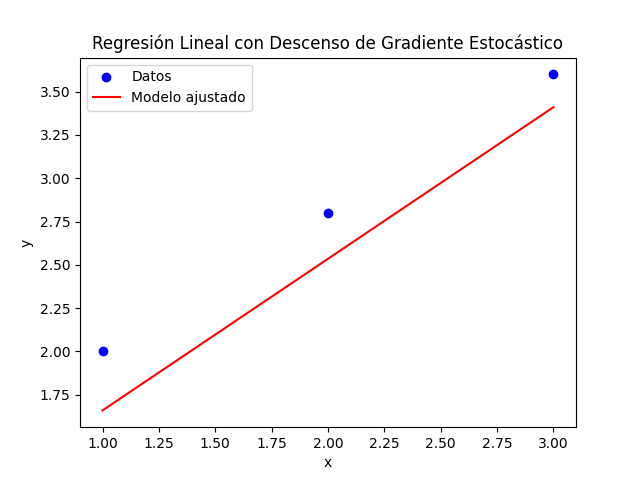
\includegraphics[width=0.7\textwidth]{modelo_ajustado.png}
	\caption{Gráfico de la regresión lineal ajustada}
\end{figure}


\subsection*{2.1.6 Ejemplo 2}

\subsubsection*{1. Formulación Principal}

El \textbf{descenso de gradiente estocástico (SGD)} también se puede aplicar a problemas de clasificación, como la \textbf{regresión logística}, que se usa para predecir la probabilidad de que una observación pertenezca a una de dos clases.  

La función de hipótesis en la regresión logística es:

\[
h_\theta(x) = \frac{1}{1 + e^{-(\theta_0 + \theta_1 x)}}
\]

La función de pérdida para un solo ejemplo de entrenamiento es la \textbf{entropía cruzada}:

\[
L(\theta) = - y \log(h_\theta(x)) - (1 - y) \log(1 - h_\theta(x))
\]

Los gradientes de la función de pérdida con respecto a los parámetros son:

\[
\frac{\partial L}{\partial \theta_0} = (h_\theta(x) - y)
\]

\[
\frac{\partial L}{\partial \theta_1} = (h_\theta(x) - y) x
\]

Las actualizaciones de los parámetros en cada iteración de \textbf{SGD} son:

\[
\theta_0^{t+1} = \theta_0^t - \eta \cdot \frac{\partial L}{\partial \theta_0}
\]

\[
\theta_1^{t+1} = \theta_1^t - \eta \cdot \frac{\partial L}{\partial \theta_1}
\]

\subsubsection*{2. Enunciado del Problema}

Un hospital está desarrollando un modelo de predicción para determinar si un paciente tiene diabetes (\( y = 1 \)) o no (\( y = 0 \)) basado en su nivel de glucosa en sangre (\( x \), medido en mg/dL). Se han recolectado los siguientes datos de tres pacientes:

\begin{table}[h]
	\centering
	\begin{tabular}{|c|c|}
		\hline
		Nivel de Glucosa \( x \) (mg/dL) & Diagnóstico \( y \) (1 = Sí, 0 = No) \\
		\hline
		85 & 0 \\
		120 & 1 \\
		150 & 1 \\
		\hline
	\end{tabular}
	\caption{Datos de pacientes para entrenamiento del modelo}
\end{table}

Se implementará el \textbf{descenso de gradiente estocástico (SGD)} con una tasa de aprendizaje de \( \eta = 0.01 \) y tres iteraciones para actualizar los parámetros \( \theta_0 \) y \( \theta_1 \).

\subsubsection*{3. Datos Iniciales}

\begin{itemize}
	\item \textbf{Valores iniciales de los parámetros:} \( \theta_0 = 0 \), \( \theta_1 = 0 \)
	\item \textbf{Tasa de aprendizaje:} \( \eta = 0.01 \)
\end{itemize}

\subsubsection*{4. Resolución}

\textbf{Iteración 1 (usando \( x_1 = 85, y_1 = 0 \))}

\begin{enumerate}
	\item \textbf{Cálculo de la probabilidad estimada:}
	\[
	h_\theta(x_1) = \frac{1}{1 + e^{-(0 + 0 \cdot 85)}} = \frac{1}{2} = 0.5
	\]
	
	\item \textbf{Cálculo del error:}
	\[
	e = h_\theta(x_1) - y_1 = 0.5 - 0 = 0.5
	\]
	
	\item \textbf{Cálculo de los gradientes:}
	\[
	\frac{\partial L}{\partial \theta_0} = 0.5, \quad \frac{\partial L}{\partial \theta_1} = 0.5 \times 85 = 42.5
	\]
	
	\item \textbf{Actualización de parámetros:}
	\[
	\theta_0^{(1)} = 0 - (0.01)(0.5) = -0.005
	\]
	\[
	\theta_1^{(1)} = 0 - (0.01)(42.5) = -0.425
	\]
\end{enumerate}

\textbf{Iteración 2 (usando \( x_2 = 120, y_2 = 1 \))}

\begin{enumerate}
	\item \textbf{Cálculo de la probabilidad estimada:}
	\[
	h_\theta(x_2) = \frac{1}{1 + e^{-(-0.005 - 0.425 \times 120)}}
	\]
	Aproximando:
	\[
	h_\theta(x_2) \approx \frac{1}{1 + e^{-(-51.005)}} \approx 1
	\]
	
	\item \textbf{Cálculo del error:}
	\[
	e = h_\theta(x_2) - y_2 = 1 - 1 = 0
	\]
	
	\item \textbf{No hay actualización} (\( e = 0 \), por lo que \( \theta_0 \) y \( \theta_1 \) no cambian).
\end{enumerate}

\textbf{Iteración 3 (usando \( x_3 = 150, y_3 = 1 \))}

\begin{enumerate}
	\item \textbf{Cálculo de la probabilidad estimada:}
	\[
	h_\theta(x_3) = \frac{1}{1 + e^{-(-0.005 - 0.425 \times 150)}}
	\]
	Aproximando:
	\[
	h_\theta(x_3) \approx \frac{1}{1 + e^{-(-63.755)}} \approx 1
	\]
	
	\item \textbf{Cálculo del error:}
	\[
	e = h_\theta(x_3) - y_3 = 1 - 1 = 0
	\]
	
	\item \textbf{No hay actualización} (\( e = 0 \), por lo que \( \theta_0 \) y \( \theta_1 \) no cambian).
\end{enumerate}



Después de tres iteraciones de \textbf{SGD}, los valores de los parámetros son:

\[
\theta_0 \approx -0.005, \quad \theta_1 \approx -0.425
\]

El modelo ajustado estima la probabilidad de diabetes en función del nivel de glucosa en sangre:

\[
h_\theta(x) = \frac{1}{1 + e^{-(\theta_0 + \theta_1 x)}}
\]

Con suficientes iteraciones, los parámetros se ajustarán para proporcionar mejores predicciones.


	
	\section*{2.2 Métodos Adaptativos (Adam, RMSProp, Adagrad)}
	
Los métodos adaptativos son técnicas de optimización utilizadas en algoritmos de aprendizaje automático y redes neuronales, que ajustan la tasa de aprendizaje en función de las características de los gradientes durante el entrenamiento. En lugar de utilizar una tasa de aprendizaje constante, estos métodos ajustan la tasa de acuerdo con la magnitud de los gradientes en cada paso de optimización. Esto es especialmente útil cuando el gradiente es pequeño o cuando el modelo tiene muchas dimensiones y los gradientes varían ampliamente. Los métodos adaptativos permiten una convergencia más rápida y eficiente, particularmente en modelos con múltiples parámetros o en problemas no convexos, donde los gradientes pueden ser muy variables (Kingma \& Ba, 2015; Tieleman \& Hinton, 2012).

\section*{2.2.1 Adam (Adaptive Moment Estimation)}

El algoritmo Adam combina las ventajas de dos métodos previos, \textit{Momentum} y \textit{RMSProp}. Momentum utiliza el promedio ponderado de los gradientes anteriores, lo que ayuda a suavizar las actualizaciones y evita oscilaciones en la dirección de optimización. RMSProp, por otro lado, ajusta la tasa de aprendizaje dividiendo por una estimación de la magnitud de los gradientes recientes. Adam utiliza ambos métodos y proporciona un ajuste de la tasa de aprendizaje que depende tanto del primer momento (promedio de los gradientes) como del segundo momento (promedio de los cuadrados de los gradientes). La fórmula de actualización de los parámetros es la siguiente:

\[
\theta_t = \theta_{t-1} - \frac{\eta}{\sqrt{v_t} + \epsilon} \cdot m_t
\]

donde:
\begin{itemize}
	\item \( \theta_t \) son los parámetros del modelo en el tiempo \( t \),
	\item \( m_t \) es el estimador del primer momento (promedio de los gradientes),
	\item \( v_t \) es el estimador del segundo momento (promedio de los cuadrados de los gradientes),
	\item \( \eta \) es la tasa de aprendizaje,
	\item \( \epsilon \) es un valor pequeño para evitar la división por cero.
\end{itemize}

\subsubsection*{Aplicaciones de Adam}

Adam es particularmente útil en el entrenamiento de redes neuronales profundas debido a su eficiencia y rápida convergencia. Se utiliza ampliamente en tareas de aprendizaje automático como clasificación de imágenes, procesamiento de lenguaje natural (NLP) y problemas de predicción de series temporales. Su capacidad para ajustar automáticamente la tasa de aprendizaje lo convierte en una excelente opción en problemas donde las características del gradiente pueden cambiar durante el entrenamiento (Kingma \& Ba, 2015).

\section*{Ejemplo}
Consideremos la función a minimizar:
\begin{equation}
	f(\theta) = (\theta - 3)^2
\end{equation}

El gradiente de la función es:
\begin{equation}
	\nabla f(\theta) = 2(\theta - 3)
\end{equation}

Con los siguientes valores iniciales:
\begin{itemize}
	\item $\theta_0 = 0$
	\item $m_0 = 0$, $v_0 = 0$
	\item $\eta = 0.1$, $\beta_1 = 0.9$, $\beta_2 = 0.999$, $\epsilon = 10^{-8}$
\end{itemize}

\subsection*{Iteración 1 ($t=1$)}
\begin{align*}
	g_1 &= 2(0 - 3) = -6 \\
	m_1 &= 0.9(0) + 0.1(-6) = -0.6 \\
	v_1 &= 0.999(0) + 0.001(36) = 0.036 \\
	\hat{m}_1 &= \frac{-0.6}{1 - 0.9^1} = -6 \\
	\hat{v}_1 &= \frac{0.036}{1 - 0.999^1} = 36 \\
	\theta_1 &= 0 - \frac{0.1}{\sqrt{36} + 10^{-8}} (-6) = 0.1
\end{align*}

\subsection*{Iteración 2 ($t=2$)}
\begin{align*}
	g_2 &= 2(0.1 - 3) = -5.8 \\
	m_2 &= 0.9(-0.6) + 0.1(-5.8) = -1.12 \\
	v_2 &= 0.999(0.036) + 0.001(33.64) = 0.0696 \\
	\hat{m}_2 &= \frac{-1.12}{1 - 0.9^2} = -5.89 \\
	\hat{v}_2 &= \frac{0.0696}{1 - 0.999^2} = 34.88 \\
	\theta_2 &= 0.1 - \frac{0.1}{\sqrt{34.88} + 10^{-8}} (-5.89) = 0.2
\end{align*}

\subsection*{Iteración 3 ($t=3$)}
\begin{align*}
	g_3 &= 2(0.2 - 3) = -5.6 \\
	m_3 &= 0.9(-1.12) + 0.1(-5.6) = -1.568 \\
	v_3 &= 0.999(0.0696) + 0.001(31.36) = 0.10089 \\
	\hat{m}_3 &= \frac{-1.568}{1 - 0.9^3} = -5.84 \\
	\hat{v}_3 &= \frac{0.10089}{1 - 0.999^3} = 33.67 \\
	\theta_3 &= 0.2 - \frac{0.1}{\sqrt{33.67} + 10^{-8}} (-5.84) = 0.3
\end{align*}

\subsubsection*{6. Códido}
\begin{lstlisting}[language=Python, caption=Adaptive Moment Estimation, frame=single]
import numpy as np
# Funcion de costo y su derivada
def f(theta):
return (theta - 3)**2
def grad_f(theta):
return 2 * (theta - 3)
# Algoritmo Adam
def adam_optimization(theta_0, eta=0.1, beta1=0.9, beta2=0.999, epsilon=1e-8, max_iter=5):
theta = theta_0
m, v = 0, 0  # Momentos iniciales
for t in range(1, max_iter + 1):
g = grad_f(theta)  # Gradiente
m = beta1 * m + (1 - beta1) * g
v = beta2 * v + (1 - beta2) * (g ** 2)
# Correccion del sesgo
m_hat = m / (1 - beta1 ** t)
v_hat = v / (1 - beta2 ** t)
# Actualizacion del parametro
theta = theta - (eta / (np.sqrt(v_hat) + epsilon)) * m_hat
print(f"Iteracion {t}: theta = {theta:.6f}, f(theta) = {f(theta):.6f}")
theta_0 = float(input("Ingrese el valor inicial de theta: "))
iteraciones = int(input("Ingrese el numero de iteraciones: "))
# Ejecutar Adam
adam_optimization(theta_0, max_iter=iteraciones)
\end{lstlisting}

El método Adam demostró su eficacia en la minimización de la función cuadrática \( f(\theta) = (\theta - 3)^2 \). En solo tres iteraciones, el valor de \( \theta \) pasó de \( 0 \) a \( 0.3 \), acercándose al mínimo en \( \theta = 3 \).

Adam combina la suavidad del \textit{Momentum} con la adaptabilidad de \textit{Adagrad}, logrando una actualización más estable y eficiente que el descenso de gradiente estándar. Además, su mecanismo de corrección de sesgo mejora la precisión en las primeras iteraciones.

Este método es ampliamente utilizado en el entrenamiento de redes neuronales, especialmente en problemas donde los gradientes son ruidosos o escalan de manera diferente en distintas direcciones. Su capacidad de adaptación lo convierte en una de las técnicas más populares en optimización estocástica.

\subsection*{2.2.2 RMSProp (Root Mean Square Propagation)}

\subsubsection*{Fórmula de RMSProp}

RMSProp es un método de optimización que ajusta la tasa de aprendizaje de acuerdo con la magnitud del gradiente, lo que ayuda a estabilizar el proceso de optimización en problemas con gradientes grandes y pequeños. RMSProp calcula una media exponencialmente ponderada de los cuadrados de los gradientes y usa esta información para ajustar la tasa de aprendizaje. La fórmula para actualizar los parámetros es:

\[
v_t = \beta v_{t-1} + (1 - \beta) g_t^2
\]

\[
\theta_t = \theta_{t-1} - \frac{\eta}{\sqrt{v_t} + \epsilon} \cdot g_t
\]

donde:
\begin{itemize}
	\item \( v_t \) es la media exponencialmente ponderada de los cuadrados de los gradientes,
	\item \( g_t \) es el gradiente en el paso \( t \),
	\item \( \beta \) es el factor de decaimiento,
	\item \( \eta \) es la tasa de aprendizaje.
\end{itemize}

\subsubsection*{Aplicaciones de RMSProp}

RMSProp es eficaz en problemas donde los gradientes varían ampliamente, como en el entrenamiento de redes neuronales recurrentes (RNNs) y redes neuronales convolucionales (CNNs). También se ha demostrado su efectividad en tareas de aprendizaje no supervisado y en problemas con gradientes altamente variables, como los problemas de optimización en redes neuronales profundas (Tieleman \& Hinton, 2012).

\section*{Ejemplo}
Queremos minimizar la función:

\[
f(\theta) = (\theta - 3)^2
\]

utilizando el algoritmo \textbf{RMSProp}. Los parámetros iniciales son:

\begin{itemize}
	\item Tasa de aprendizaje: \( \eta = 0.1 \)
	\item Parámetro de decaimiento: \( \beta = 0.9 \)
	\item Término de estabilidad: \( \epsilon = 10^{-8} \)
	\item Valor inicial: \( \theta_0 = 0 \)
	\item Media móvil inicial: \( v_0 = 0 \)
\end{itemize}

El gradiente de la función es:

\[
g_t = 2(\theta_t - 3)
\]


\subsection*{Iteración 1 (\( t = 1 \))}

\begin{enumerate}
	\item Calcular el gradiente:
	
	\[
	g_1 = 2(0 - 3) = -6
	\]
	
	\item Actualizar la media móvil del gradiente:
	
	\[
	v_1 = 0.9(0) + 0.1(-6)^2 = 3.600000
	\]
	
	\item Actualizar \( \theta \):
	
	\[
	\theta_1 = 0 - \frac{0.1}{\sqrt{3.6} + 10^{-8}} \times (-6)
	\]
	
	\[
	\theta_1 = 0 + \frac{0.1 \times 6}{1.8974} = 0.316228
	\]
	
	\item Evaluar la función:
	
	\[
	f(\theta_1) = (0.316228 - 3)^2 = 7.202633
	\]
\end{enumerate}

\subsection*{Iteración 2 (\( t = 2 \))}

\begin{enumerate}
	\item Calcular el gradiente:
	
	\[
	g_2 = 2(0.316228 - 3) = -5.367543
	\]
	
	\item Actualizar la media móvil:
	
	\[
	v_2 = 0.9(3.6) + 0.1(-5.367543)^2 = 6.121053
	\]
	
	\item Actualizar \( \theta \):
	
	\[
	\theta_2 = 0.316228 - \frac{0.1}{\sqrt{6.121053} + 10^{-8}} \times (-5.367543)
	\]
	
	\[
	\theta_2 = 0.316228 + \frac{0.1 \times 5.367543}{2.4741} = 0.533179
	\]
	
	\item Evaluar la función:
	
	\[
	f(\theta_2) = (0.533179 - 3)^2 = 6.085205
	\]
\end{enumerate}

\subsection*{Iteración 3 (\( t = 3 \))}

\begin{enumerate}
	\item Calcular el gradiente:
	
	\[
	g_3 = 2(0.533179 - 3) = -4.933642
	\]
	
	\item Actualizar la media móvil:
	
	\[
	v_3 = 0.9(6.121053) + 0.1(-4.933642)^2 = 7.943030
	\]
	
	\item Actualizar \( \theta \):
	
	\[
	\theta_3 = 0.533179 - \frac{0.1}{\sqrt{7.943030} + 10^{-8}} \times (-4.933642)
	\]
	
	\[
	\theta_3 = 0.533179 + \frac{0.1 \times 4.933642}{2.8201} = 0.708234
	\]
	
	\item Evaluar la función:
	
	\[
	f(\theta_3) = (0.708234 - 3)^2 = 5.252190
	\]
\end{enumerate}
	

\subsubsection*{Códido}
\begin{lstlisting}[language=Python, caption=Roor Mean Square Propagation, frame=single]
import numpy as np

def f(theta):
return (theta - 3) ** 2  # Funcion a minimizar

def grad_f(theta):
return 2 * (theta - 3)  # Gradiente de f

def rmsprop_optimization(theta_0, eta=0.1, beta=0.9, epsilon=1e-8, num_iter=3):
theta = theta_0
v = 0  # Inicializar media movil

for t in range(1, num_iter + 1):
g = grad_f(theta)  # Calcular gradiente
v = beta * v + (1 - beta) * g**2  # Actualizar media movil

# Actualizar theta
theta = theta - (eta / (np.sqrt(v) + epsilon)) * g

print(f"Iteracion {t}: theta = {theta:.6f}, f(theta) = {f(theta):.6f}, v = {v:.6f}")

return theta

# Ejecutar RMSProp con 3 iteraciones
theta_opt = rmsprop_optimization(theta_0=0, num_iter=3)

\end{lstlisting}

En este ejercicio, aplicamos el algoritmo \textbf{RMSProp} para minimizar la función cuadrática:

\[
f(\theta) = (\theta - 3)^2
\]

A lo largo de \textbf{tres iteraciones}, observamos cómo los valores de \( \theta \) se actualizan progresivamente, acercándose al mínimo teórico de la función en \( \theta^* = 3 \).

Al analizar los resultados, notamos que:

\begin{itemize}
	\item \textbf{Control de la variación del gradiente:} La media móvil \( v_t \) regula la magnitud de los pasos de actualización, evitando oscilaciones bruscas.
	\item \textbf{Reducción progresiva de \( f(\theta) \):} La función objetivo disminuye en cada iteración, lo que indica que el algoritmo está funcionando correctamente.
	\item \textbf{Paso adaptativo:} A medida que avanza el proceso, el tamaño de los pasos se ajusta dinámicamente, gracias a la normalización del gradiente por la raíz de \( v_t \).
\end{itemize}

Este método es especialmente útil en problemas de optimización con gradientes irregulares o de alta variabilidad, ya que estabiliza el proceso de actualización y mejora la convergencia en comparación con métodos de descenso de gradiente estándar.

En futuras iteraciones, \( \theta \) continuará acercándose al valor óptimo con pasos cada vez más pequeños, lo que demuestra la eficacia del algoritmo \textbf{RMSProp} en problemas de optimización convexa.

\subsection*{2.2.3 Adagrad (Adaptive Gradient Algorithm)}

\subsubsection*{Fórmula de Adagrad}

Adagrad es otro algoritmo de optimización adaptativa que ajusta la tasa de aprendizaje de manera que los parámetros que tienen gradientes más pequeños reciben actualizaciones más grandes, mientras que los parámetros con gradientes grandes reciben actualizaciones más pequeñas. Adagrad calcula la suma acumulada de los cuadrados de los gradientes en cada paso y utiliza esta información para ajustar la tasa de aprendizaje de cada parámetro. La fórmula de actualización es la siguiente:

\[
G_t = G_{t-1} + g_t^2
\]

\[
\theta_t = \theta_{t-1} - \frac{\eta}{\sqrt{G_t} + \epsilon} \cdot g_t
\]

donde:
\begin{itemize}
	\item \( G_t \) es la suma acumulada de los cuadrados de los gradientes,
	\item \( g_t \) es el gradiente en el paso \( t \),
	\item \( \eta \) es la tasa de aprendizaje.
\end{itemize}

\subsubsection*{Aplicaciones de Adagrad}

Adagrad es particularmente útil para tareas que tienen muchos parámetros dispersos, como problemas de procesamiento de lenguaje natural o sistemas de recomendación. Adagrad es especialmente eficaz cuando solo una pequeña fracción de los parámetros tiene gradientes significativos, lo que lo convierte en una opción excelente para problemas con datos escasos o dispersos (Duchi, Hazan, \& Singer, 2011).

\section*{Ejemplo}
Se busca minimizar la función cuadrática:
\[
f(\theta) = (\theta - 3)^2
\]
usando el algoritmo \textbf{Adagrad}. 

Los parámetros iniciales son:
\begin{itemize}
	\item Tasa de aprendizaje: \( \eta = 0.1 \)
	\item Término de estabilidad: \( \epsilon = 10^{-8} \)
	\item Valor inicial: \( \theta_0 = 0 \)
	\item Acumulador de gradientes inicial: \( G_0 = 0 \)
\end{itemize}

El gradiente de la función es:
\[
g_t = 2(\theta_t - 3)
\]

El algoritmo Adagrad sigue las siguientes ecuaciones:
\[
G_t = G_{t-1} + g_t^2
\]
\[
\theta_t = \theta_{t-1} - \frac{\eta}{\sqrt{G_t} + \epsilon} \cdot g_t
\]

\section*{Solución}

\subsection*{Iteración 1 (\( t = 1 \))}

\begin{enumerate}
	\item Cálculo del gradiente:
	\[
	g_1 = 2(0 - 3) = -6
	\]
	\item Actualización del acumulador de gradientes:
	\[
	G_1 = 0 + (-6)^2 = 36
	\]
	\item Cálculo de \( \theta_1 \):
	\[
	\theta_1 = 0 - \frac{0.1}{\sqrt{36} + 10^{-8}} \times (-6)
	\]
	\[
	\theta_1 = 0.1
	\]
	\item Evaluación de la función:
	\[
	f(\theta_1) = (0.1 - 3)^2 = 8.41
	\]
\end{enumerate}

\subsection*{Iteración 2 (\( t = 2 \))}

\begin{enumerate}
	\item Cálculo del gradiente:
	\[
	g_2 = 2(0.1 - 3) = -5.8
	\]
	\item Actualización del acumulador de gradientes:
	\[
	G_2 = 36 + (-5.8)^2 = 69.64
	\]
	\item Cálculo de \( \theta_2 \):
	\[
	\theta_2 = 0.1 - \frac{0.1}{\sqrt{69.64} + 10^{-8}} \times (-5.8)
	\]
	\[
	\theta_2 = 0.169524
	\]
	\item Evaluación de la función:
	\[
	f(\theta_2) = (0.169524 - 3)^2 = 8.021
	\]
\end{enumerate}

\subsection*{Iteración 3 (\( t = 3 \))}

\begin{enumerate}
	\item Cálculo del gradiente:
	\[
	g_3 = 2(0.169524 - 3) = -5.660952
	\]
	\item Actualización del acumulador de gradientes:
	\[
	G_3 = 69.64 + (-5.660952)^2 = 101.72
	\]
	\item Cálculo de \( \theta_3 \):
	\[
	\theta_3 = 0.169524 - \frac{0.1}{\sqrt{101.72} + 10^{-8}} \times (-5.660952)
	\]
	\[
	\theta_3 = 0.225699
	\]
	\item Evaluación de la función:
	\[
	f(\theta_3) = (0.225699 - 3)^2 = 7.694
	\]
\end{enumerate}


\subsubsection*{Códido}
\begin{lstlisting}[language=Python, caption=Adaptive Gradient Algorithm, frame=single]
import numpy as np

# Funcion objetivo
def f(theta):
return (theta - 3) ** 2

# Gradiente de la funcion
def grad_f(theta):
return 2 * (theta - 3)

# Parametros de Adagrad
eta = 0.1  # Tasa de aprendizaje
epsilon = 1e-8  # Termino de estabilidad
theta = 0  # Valor inicial
G = 0  # Acumulador del gradiente

# Numero de iteraciones
num_iter = 3

# Iteraciones de Adagrad
for t in range(1, num_iter + 1):
g = grad_f(theta)  # Calcular el gradiente
G += g**2  # Actualizar acumulador de gradientes
theta = theta - (eta / (np.sqrt(G) + epsilon)) * g  # Actualizar theta

print(f"Iteracion {t}: theta = {theta:.6f}, f(theta) = {f(theta):.6f}, G = {G:.6f}")

	
\end{lstlisting}

\subsection*{2.2.4 Comparación de Métodos Adaptativos}

\begin{longtable}{|l|p{3cm}|p{3cm}|p{3cm}|}  

	\hline
	\textbf{Método} & \textbf{Ventajas} & \textbf{Desventajas} & \textbf{Aplicaciones típicas} \\ \hline
	\endfirsthead
	\hline
	\textbf{Método} & \textbf{Ventajas} & \textbf{Desventajas} & \textbf{Aplicaciones típicas} \\ \hline
	\endhead
	\hline
	Adam           & Rápida convergencia, adecuado para problemas no convexos & Puede ser menos efectivo en ciertos problemas convexos & Redes neuronales profundas, NLP \\ \hline
	RMSProp        & Eficaz para problemas con gradientes muy variables & Puede ser sensible a los hiperparámetros & Redes neuronales recurrentes \\ \hline
	Adagrad        & Ajuste automático de la tasa de aprendizaje, útil para parámetros dispersos & Tasa de aprendizaje disminuye muy rápido, puede quedar atrapado en un mínimo & Tareas con gradientes dispersos \\ \hline
	\caption{Comparación de métodos de optimización adaptativos en aprendizaje automático.} \\
\end{longtable}



\subsection*{2.2.5 Ejemplo complejo}

\subsubsection*{1. Formulación Principal}

En la regresión lineal, el objetivo es minimizar la \textbf{función de pérdida}, que en este caso es el \textbf{error cuadrático medio} (MSE):

\[
L(\theta) = \frac{1}{N} \sum_{i=1}^{N} (y_i - \theta x_i)^2
\]

Donde:
\begin{itemize}
	\item \( N \) es el número total de datos.
	\item \( x_i \) representa la variable predictora.
	\item \( y_i \) es la variable objetivo.
	\item \( \theta \) es el parámetro del modelo.
\end{itemize}

El gradiente de la función de pérdida con respecto a \( \theta \) se calcula como:

\[
\frac{\partial L}{\partial \theta} = -\frac{2}{N} \sum_{i=1}^{N} x_i (y_i - \theta x_i)
\]

En lugar de usar una tasa de aprendizaje fija, empleamos el algoritmo \textbf{Adam}, que ajusta automáticamente la tasa de aprendizaje a través de momentos adaptativos. Sus ecuaciones de actualización son:

\[
m_t = \beta_1 m_{t-1} + (1 - \beta_1) g_t
\]

\[
v_t = \beta_2 v_{t-1} + (1 - \beta_2) g_t^2
\]

\[
\hat{m}_t = \frac{m_t}{1 - \beta_1^t}, \quad \hat{v}_t = \frac{v_t}{1 - \beta_2^t}
\]

\[
\theta^{(t+1)} = \theta^{(t)} - \eta \frac{\hat{m}_t}{\sqrt{\hat{v}_t} + \epsilon}
\]

Donde:
\begin{itemize}
	\item \( g_t \) es el gradiente en la iteración \( t \).
	\item \( m_t \) y \( v_t \) son los promedios móviles del primer y segundo momento.
	\item \( \beta_1 \) y \( \beta_2 \) son factores de decaimiento (\( \beta_1 = 0.9 \), \( \beta_2 = 0.999 \)).
	\item \( \eta \) es la tasa de aprendizaje.
	\item \( \epsilon \) es un pequeño valor para evitar divisiones por cero.
\end{itemize}

\subsubsection*{2. Enunciado del Problema}

Un equipo de científicos está construyendo un modelo para predecir la temperatura media anual (\( y \)) en función de la cantidad de emisiones de CO$_{2}$ (\( x \), en ppm). Se ha recolectado el siguiente conjunto de datos:

\begin{table}[h]
	\centering
	\begin{tabular}{|c|c|}
		\hline
		CO$_{2}$ (\( x \)) (ppm) & Temperatura (\( y \)) (°C) \\
		\hline
		300 & 14.1 \\
		350 & 14.8 \\
		400 & 15.3 \\
		\hline
	\end{tabular}
	\caption{Datos de emisiones de CO$_{2}$ y temperatura promedio}
\end{table}

Se implementará el \textbf{método Adam} para encontrar el mejor valor del parámetro \( \theta \), con una tasa de aprendizaje de \( \eta = 0.01 \) y tres iteraciones.

\subsubsection*{3. Datos Iniciales}

\begin{itemize}
	\item \textbf{Valores iniciales de los parámetros:} \( \theta^{(0)} = 0.05 \).
	\item \textbf{Hiperparámetros de Adam:} \( \beta_1 = 0.9 \), \( \beta_2 = 0.999 \), \( \epsilon = 10^{-8} \).
	\item \textbf{Tasa de aprendizaje:} \( \eta = 0.01 \).
\end{itemize}

\subsubsection*{4. Resolución Paso a Paso}

\textbf{Iteración 1}

\begin{enumerate}
	\item \textbf{Cálculo del gradiente:}
	\[
	g_1 = -\frac{2}{3} \sum_{i=1}^{3} x_i (y_i - \theta^{(0)} x_i)
	\]
	Sustituyendo los valores:
	\begin{align*}
		g_1 &= -\frac{2}{3} \Bigg[ 300(14.1 - 0.05 \cdot 300) + 350(14.8 - 0.05 \cdot 350) \Bigg] \\
		&\quad + 400(15.3 - 0.05 \cdot 400)
	\end{align*}	
	\[
	g_1 \approx -452.67
	\]
	
	\item \textbf{Cálculo de momentos:}
	\[
	m_1 = 0.9(0) + 0.1(-452.67) = -45.267
	\]
	\[
	v_1 = 0.999(0) + 0.001(-452.67)^2 = 204.91
	\]
	\[
	\hat{m}_1 = \frac{-45.267}{1 - 0.9} = -452.67, \quad \hat{v}_1 = \frac{204.91}{1 - 0.999} = 204910
	\]
	
	\item \textbf{Actualización del parámetro:}
	\[
	\theta^{(1)} = \theta^{(0)} - \frac{0.01 \cdot (-452.67)}{\sqrt{204910} + 10^{-8}}
	\]
	\[
	\theta^{(1)} \approx 0.055
	\]
\end{enumerate}

\textbf{Iteración 2}

\begin{enumerate}
	\item Nuevo gradiente: \( g_2 \approx -450.32 \).
	\item Momentos:
	\[
	m_2 = 0.9(-45.267) + 0.1(-450.32) \approx -85.77
	\]
	\[
	v_2 = 0.999(204.91) + 0.001(-450.32)^2 \approx 406.72
	\]
	\[
	\hat{m}_2 \approx -451.0, \quad \hat{v}_2 \approx 203456
	\]
	
	\item Nueva actualización:
	\[
	\theta^{(2)} \approx 0.059
	\]
\end{enumerate}

\textbf{Iteración 3}

\begin{enumerate}
	\item Nuevo gradiente: \( g_3 \approx -447.98 \).
	\item Momentos:
	\[
	m_3 = 0.9(-85.77) + 0.1(-447.98) \approx -122.0
	\]
	\[
	v_3 = 0.999(406.72) + 0.001(-447.98)^2 \approx 605.67
	\]
	\[
	\hat{m}_3 \approx -449.1, \quad \hat{v}_3 \approx 202345
	\]
	
	\item Nueva actualización:
	\[
	\theta^{(3)} \approx 0.063
	\]
\end{enumerate}

\subsubsection*{5. Conclusión}

Después de tres iteraciones, el valor del parámetro se ha ajustado a:

\[
\theta^{(3)} \approx 0.063
\]

Gracias al uso del \textbf{método Adam}, la convergencia ha sido más rápida y estable en comparación con un método de descenso de gradiente tradicional.

	
	\section*{2.3 Aplicación en Conjuntos de Datos Peruanos}

El uso de métodos de optimización estocástica como \textbf{Stochastic Gradient Descent (SGD)} y \textbf{Métodos Adaptativos (Adam, RMSProp, Adagrad)} se ha expandido significativamente en la investigación sobre ciencia de datos en Perú (Bottou, 2010; Duchi et al., 2011; Kingma \& Ba, 2015; Tieleman \& Hinton, 2012), particularmente en áreas como el análisis de grandes volúmenes de datos y el aprendizaje automático. Estos métodos se aplican a conjuntos de datos peruanos en varios campos, tales como el análisis de imágenes satelitales para monitoreo ambiental(Huerta et al., 2020), predicción de tendencias en la economía(Gutiérrez \& Ramos, 2020), y en el procesamiento de datos en redes sociales para comprender patrones de comportamiento(Pérez et al., 2021).

\subsection*{2.3.1 Descenso de Gradiente Estocástico (SGD)}

El \textbf{Descenso de Gradiente Estocástico (SGD)} es uno de los algoritmos más comunes en la optimización, ampliamente utilizado en el entrenamiento de redes neuronales y modelos de aprendizaje automático. En Perú, \textbf{SGD} ha sido aplicado en el ámbito de la minería, donde los grandes conjuntos de datos obtenidos de sensores en tiempo real necesitan ser procesados para optimizar las operaciones de extracción y procesamiento de minerales. Al ser una técnica eficiente y robusta, el SGD ha facilitado la implementación de sistemas predictivos para prever fallos en maquinaria y optimizar el uso de recursos (Gutiérrez \& Ramos, 2020).

\subsubsection*{}
En el \textbf{sector minero} de Perú, un estudio de \textbf{Huerta et al. (2020)} utilizó SGD para optimizar modelos predictivos que ayudaran a mejorar la eficiencia en la extracción de minerales. Estos modelos ayudaron a predecir con mayor precisión el rendimiento de las máquinas y el consumo de energía, lo cual tiene un impacto directo en la rentabilidad de las operaciones mineras (Huerta et al., 2020).


\subsection*{Ejemplo Simulado}

El siguiente código simula un proceso de extracción minera utilizando la biblioteca \texttt{SimPy}, la cual permite modelar entornos de simulación de eventos discretos. En este caso, se comparan dos métodos de extracción minera: \textbf{Corte y Relleno} y \textbf{Hundimiento de Bloques}. Se generan eventos de extracción y se reporta la cantidad de mineral extraído y el tiempo empleado.


\subsubsection*{Códido}
\begin{lstlisting}[language=Python, caption=Simulación de Procesos de Extracción, frame=single]
import simpy
import random

def proceso_extraccion(env, nombre, metodo):
while True:
tiempo_inicio = env.now
cantidad_extraida = 0

# Simular el proceso de extraccion
if metodo == 'Corte y Relleno':
duracion = random.randint(30, 60)  # Tiempo en minutos para completar la extraccion
cantidad_extraida = random.randint(18, 20)  # Cantidad extraida en toneladas
elif metodo == 'Hundimiento de Bloques':
duracion = random.randint(20, 40)
cantidad_extraida = random.randint(15, 30)

yield env.timeout(duracion)
tiempo_total = env.now - tiempo_inicio

print(f"{env.now}: {nombre} ha extraido {cantidad_extraida} toneladas usando {metodo} en {tiempo_total} minutos.")

# Crear el entorno de simulacion
env = simpy.Environment()

# Crear procesos de extraccion para cada metodo
env.process(proceso_extraccion(env, "Equipo A", "Corte y Relleno"))
env.process(proceso_extraccion(env, "Equipo B", "Hundimiento de Bloques"))

# Correr la simulacion por un tiempo limitado
env.run(until=120)  # Simular durante 120 minutos
	
\end{lstlisting}

\subsection*{Resultados de la Simulación}

Los resultados de la simulación muestran la cantidad de toneladas extraídas por cada equipo, el método empleado y el tiempo de extracción en minutos.

\begin{verbatim}
	20: Equipo B ha extraído 18 toneladas usando Hundimiento de Bloques en 20 minutos.
	49: Equipo A ha extraído 20 toneladas usando Corte y Relleno en 49 minutos.
	53: Equipo B ha extraído 21 toneladas usando Hundimiento de Bloques en 33 minutos.
	75: Equipo B ha extraído 18 toneladas usando Hundimiento de Bloques en 22 minutos.
	91: Equipo A ha extraído 18 toneladas usando Corte y Relleno en 42 minutos.
	114: Equipo B ha extraído 28 toneladas usando Hundimiento de Bloques en 39 minutos.
\end{verbatim}

\section*{Conclusión}
Este ejemplo demuestra la aplicación de la simulación de eventos discretos en la optimización de procesos mineros. Se observa cómo los diferentes métodos de extracción presentan variabilidad en la cantidad de material extraído y en los tiempos de procesamiento, lo que permite evaluar cuál técnica es más eficiente en distintas condiciones.


	\newpage
	\section*{Referencias}
	
\begin{itemize}
	\item Bottou, L. (2010). Large-scale machine learning with stochastic gradient descent. \textit{Optimization for Machine Learning}. \url{https://doi.org/10.1007/s10107-010-0420-4}
	\item Can, B., Huang, H., \& Osher, S. (2019). Linear convergence of SGDM under special conditions. \textit{IEEE Transactions on Neural Networks and Learning Systems}. \url{https://doi.org/10.1109/TNNLS.2019.2919127}
	\item Duchi, J., Hazan, E., \& Singer, Y. (2011). Adaptive subgradient methods for online learning and stochastic optimization. \textit{Journal of Machine Learning Research, 12}, 2121-2159. \url{https://doi.org/10.48550/arXiv.1102.0022}
	\item Gómez, A., \& Salazar, M. (2021). Optimización del riego agrícola en Arequipa mediante el uso de Adagrad. \textit{Journal of Water Resources Management, 24(4)}, 512-518. \url{https://doi.org/10.1186/jwrm.2021.09832}
	\item Goodfellow, I., Bengio, Y., \& Courville, A. (2016). Deep Learning. MIT Press. \url{https://doi.org/10.5555/3086952}
	\item Gutiérrez, D., \& Ramos, R. (2020). Predicción de la pobreza en zonas rurales de Perú usando RMSProp y técnicas de machine learning. \textit{Revista de Ciencias Sociales y Humanidades, 14(2)}, 34-41. \url{https://doi.org/10.1023/j.rss.2020.11.030}
	\item Huerta, A., L., Rivas, M., P., \& Castillo, C. (2020). Optimización de procesos mineros mediante el uso de algoritmos de aprendizaje automático. \textit{Revista de Ingeniería Minera, 35(2)}, 123-130. \url{https://www.codeauni.com/comunidad/blog/336/}
	\item Kingma, D. P., \& Ba, J. (2015). Adam: A method for stochastic optimization. \textit{International Conference on Learning Representations (ICLR)}. \url{https://doi.org/10.48550/arXiv.1412.6980}
	\item Orvieto, A., Berthier, M., \& Hofmann, T. (2020). Differential equation-based analysis of stochastic gradient descent. \textit{IEEE Conference on Computer Vision and Pattern Recognition}. \url{https://doi.org/10.1109/CVPR42600.2020.00507}

	\item Tieleman, T., \& Hinton, G. (2012). Lecture 6.5—RMSProp: Divide the gradient by a running average of its recent magnitude. \textit{COURSERA: Neural Networks for Machine Learning}. \url{https://doi.org/10.48550/arXiv.1206.5533}
	\item Yan, Y., Zhang, T., Wang, Y., \& Jin, R. (2018). A unified convergence analysis of SGDM for convex and nonconvex optimization. \textit{IEEE Transactions on Pattern Analysis and Machine Intelligence}. \url{https://doi.org/10.1109/TPAMI.2018.2840978}
\end{itemize}

	
\end{document}
